%!TEX root = ../thesis.tex

\fxnote[inline, nomargin]{Note that the same/similar things hold for the left boundary walk. However we do not need this. So do I mention it?}

\fxnote[inline, nomargin]{If invariant I4 (no separating 2-chords) is satisfied then we actually have a path and not only a non-crossing walk. We currently do not do this here such that other algorithms on a Fusy based core can also use this algorithm. And I might still add 1 or 2 in the final version. }



\section{The right neighbor walk of a path}
  \label{s:rightNeighbour}

  During the proof of the sweepcycle step of the algorithm we will frequently use the concept of the right neighbor walk of a path.
  Given a path $P = p_1 \ldots p_k$ in a graph $G$
  The \emph{right neighbor walk} $W$ of $P$ will consist of $p_1$ and the vertices adjacent to $p_{2}$ between $p_1$ and $p_{3}$ in the clockwise rotation at $p_{2}$ followed by the vertices between $p_{2}$ and $p_{4}$ in the rotation at $p_{3}$ and so further until we add the vertices between $p_{k-2}$ and $p_k$ in the rotation around $p_{k-1}$ and finally we finish by adding $p_k$ to $W$.
  We then remove all subsequent duplicates from $W$

  \begin{lemma}
    \label{lm:uni:neighborWalk}
    The right neighbor walk $W$ is a walk.
  \end{lemma}
  \begin{proof}
    Let $w$ and $w'$ be two subsequent vertices in $W$. We will show they are connected. We first consider the case $\braces{w, w'} \cap \braces{p_1, p_k } = \emptyset$.
    Now there are two cases. Either $(a)$ $w$ and $w'$ are vertices adjacent to some $p_i$ an thus subsequent in the rotation at $p_i$  or $(b)$ $w$ was the last vertex adjacent to some $p_i$ and thus $w'$ is the first vertex adjacent to $p_{i+1}$.

  \begin{figure}[h]
    \centering
    \begin{subfigure}[b]{0.5\linewidth}
            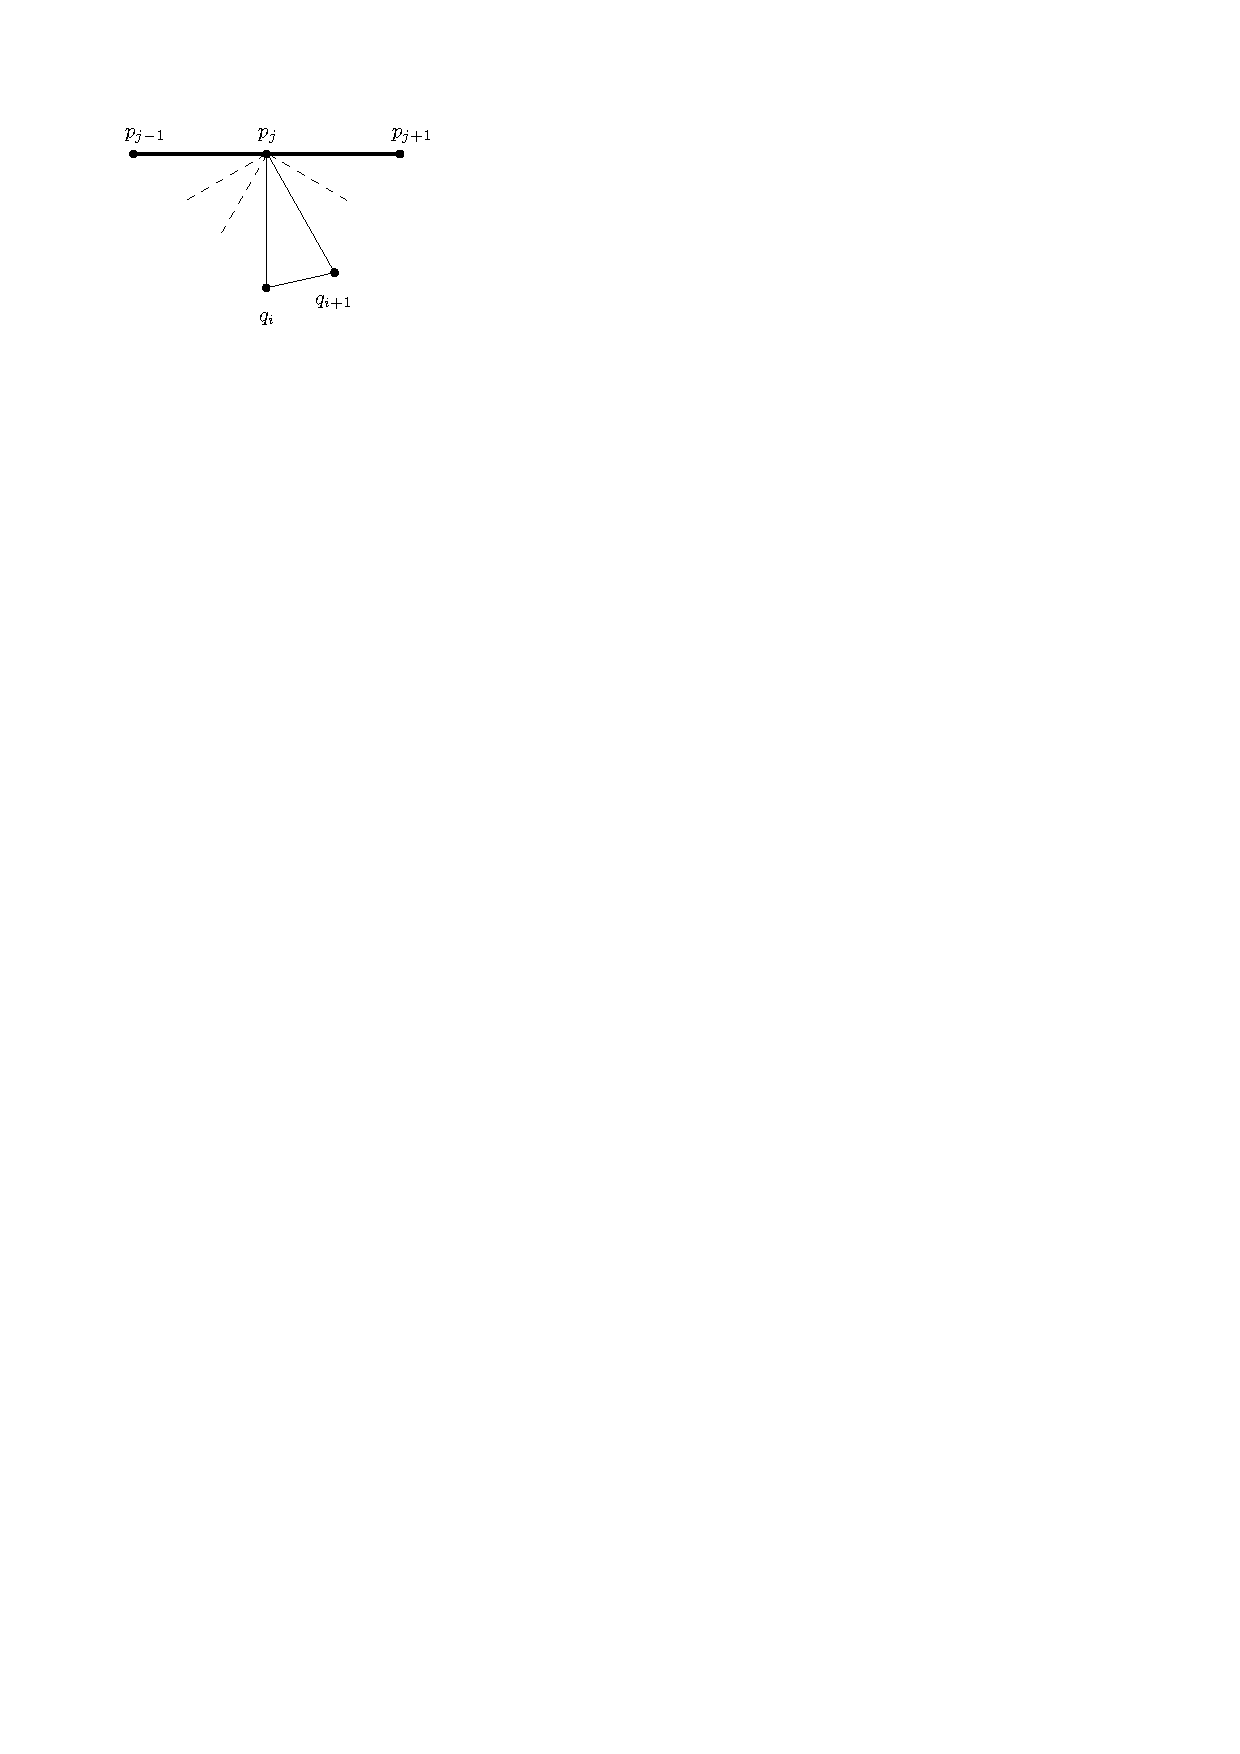
\includegraphics[width=\linewidth]{unifiedAlgo/img/walkProofA}
            \caption{}
        \end{subfigure}%
        \begin{subfigure}[b]{0.5\linewidth}
            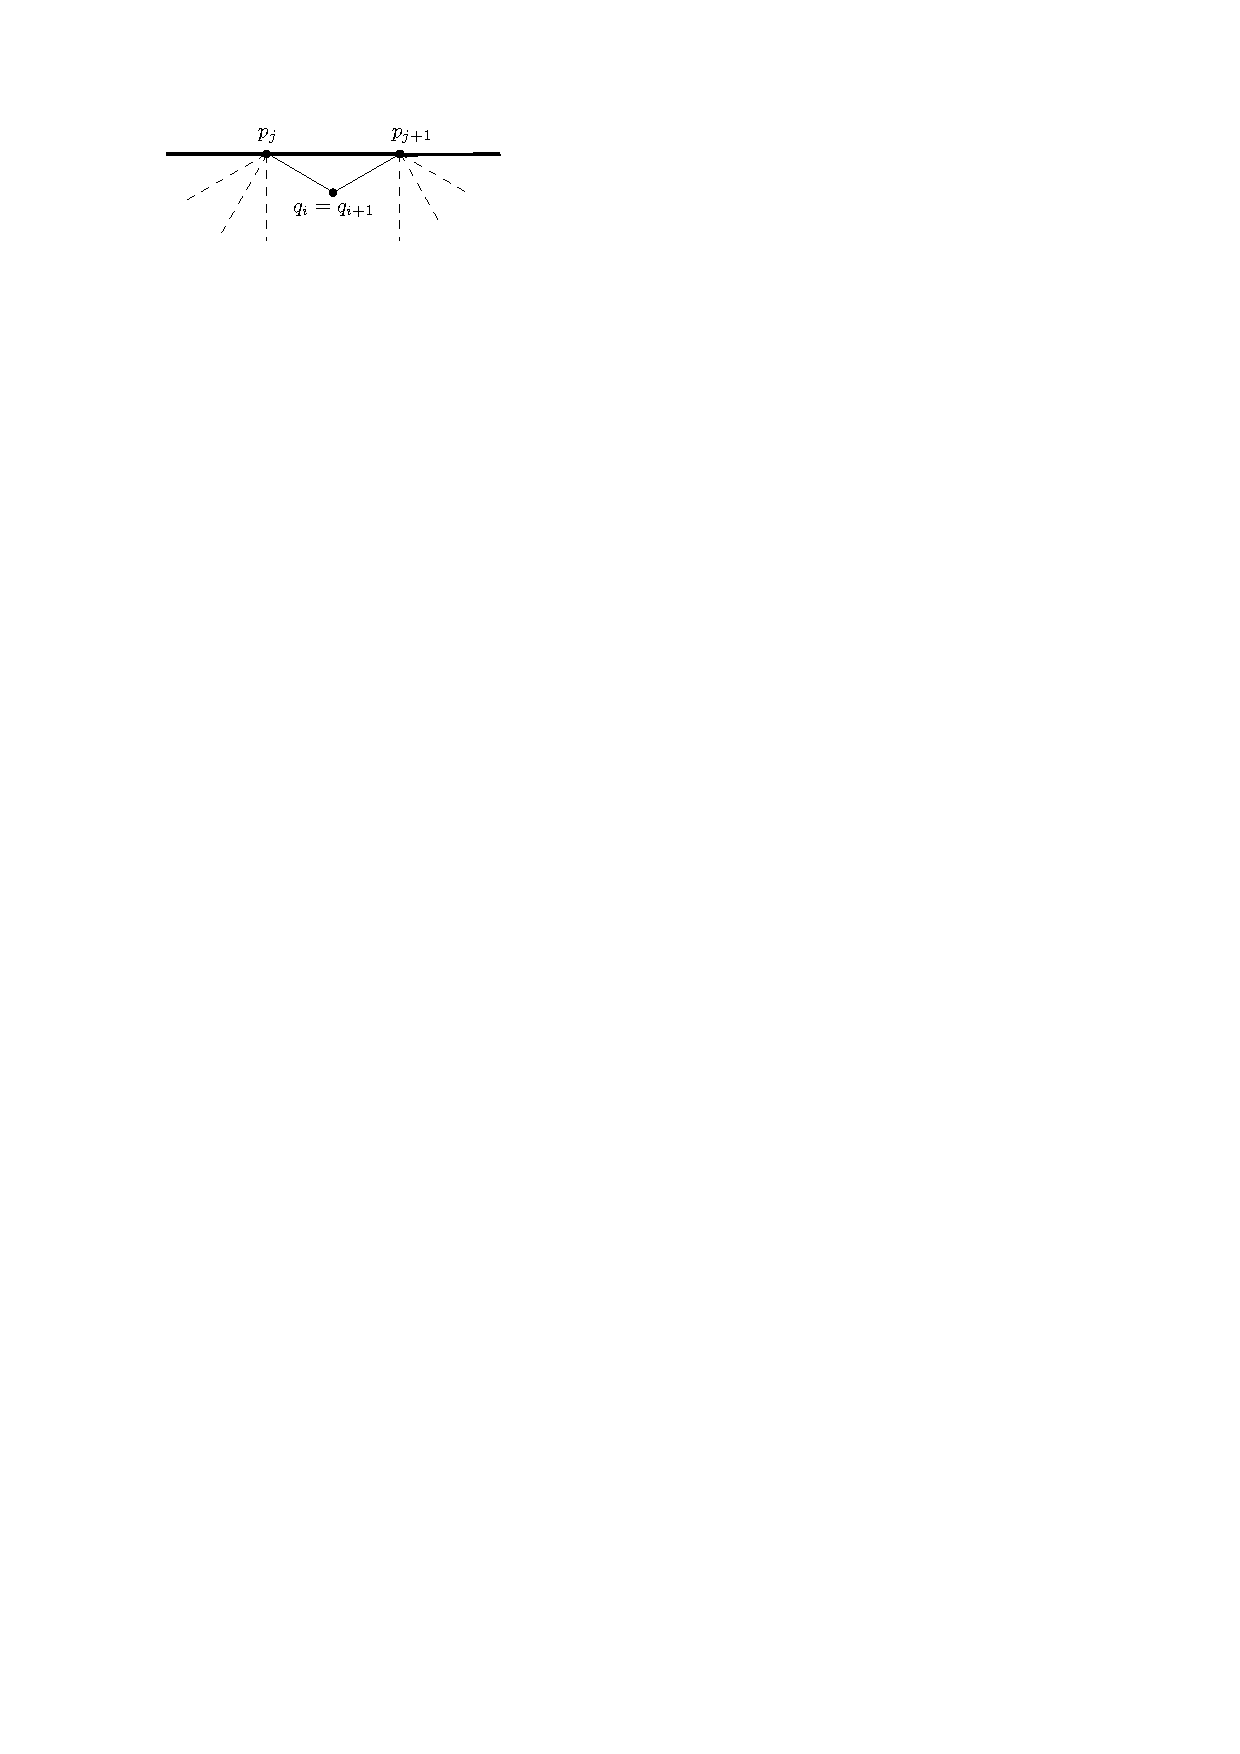
\includegraphics[width=\linewidth]{unifiedAlgo/img/walkProofB}
            \vspace{1cm}

            \caption{}
        \end{subfigure}

          \caption{The two main cases of the proof showing that $W$ is a walk}
      \label{fig:uni:walkproof}
    \end{figure}

    In case $(a)$ we note that since $w$ and $w'$ are subsequent in the rotation at $p_i$ $ww'$ is an edge since every interior face is a triangle.

    In case $(b)$ we note that $p_i w$ and $p_i p_{i+1}$ are edges subsequent in clockwise order, hence $wp_{i+1}$ is also an edge. Hence $w$ is the first vertex adjacent to $p_{i+1}$ subsequent to $v_i$ in the clockwise rotation. Thus $w= w'$. They are duplicates and one of them must have been removed.

    Now for the edge cases: Let $x$ be the first vertex adjacent to $p_{i+1}$ and let $y$ be the last vertex adjacent to $p_{j-1}$. $p_i$ and $x$ are vertices adjacent to $p_{i+1}$ subsequent in the clockwise rotation, and hence connected since every interior face is a triangle. In the same way $y$ and $v_j$ are subsequent vertices in the rotation at $v_n$ and hence connected.

    Hence $\W$ is a walk.
  \end{proof}

  \begin{lemma}
    \label{lm:uni:neighborWalkNoncrossing}
    The right neighbor walk $W$ is a non-crosssing walk.
  \end{lemma}
  \begin{proof}
    Suppose that the right neighbor walk is crossing at a vertex $w= w_i =w_j$. Then one of $w_{j-1}$ and $w_{j+1}$ is in the clockwise interval $[w_{i-1}, w_{i+1} ]$ at the rotation at the triangle containing $w$ is a separating triangle.

    We conclude that $W$ must be a non-crossing walk.
  \end{proof}


  \begin{lemma}
    \label{lm:uni:neighbourwalkNoInteriorVertex}
    The closed non-crosing walk $W \oplus \rev{P}$ has no interior vertex.
  \end{lemma}
  \begin{proof}
    The interior of $W \oplus \rev{P}$ consists of only triangles with all vertices in $W \oplus \rev{P}$. We can see this from the construction of the neighbor walk. Both cases in Figure \ref{fig:uni:walkproof} add a triangle to the interior with all vertices in $W \oplus \rev{P}$.

    Suppose there is a interior vertex. Then the triangle containing this vertex is a separating triangle.
  \end{proof}


  \begin{lemma}
    \label{lm:uni:neighbourwalkChordFree}
    The left of the of a right neighbor walk is chordfree.
  \end{lemma}
  \begin{proof}
    Suppose that the right neighbor walk $W = w_1 \ldots w_k$  has a chord on the left, say between $w_i$ and $w_j$ with $i< j -1 $. There is a vertex $p_\ell \in P$ on the path such that $w_{i+1}$ is a neighbor of $p_\ell$ to the left of $p_\ell$ Consider now the following non-crossing closed walk $P w_k \ldots w_{j+1} w_j w_i w_{i-1} \ldots w_1$
    (Thick in Figure \ref{fig:uni:neihbourwalkChordFree})this walk has $w_{i+1}$ in its exterior. But then $p_\ell w_{i+1}$ is a crossing edge. Which is forbidden.

    \begin{figure}[h]
      \centering
      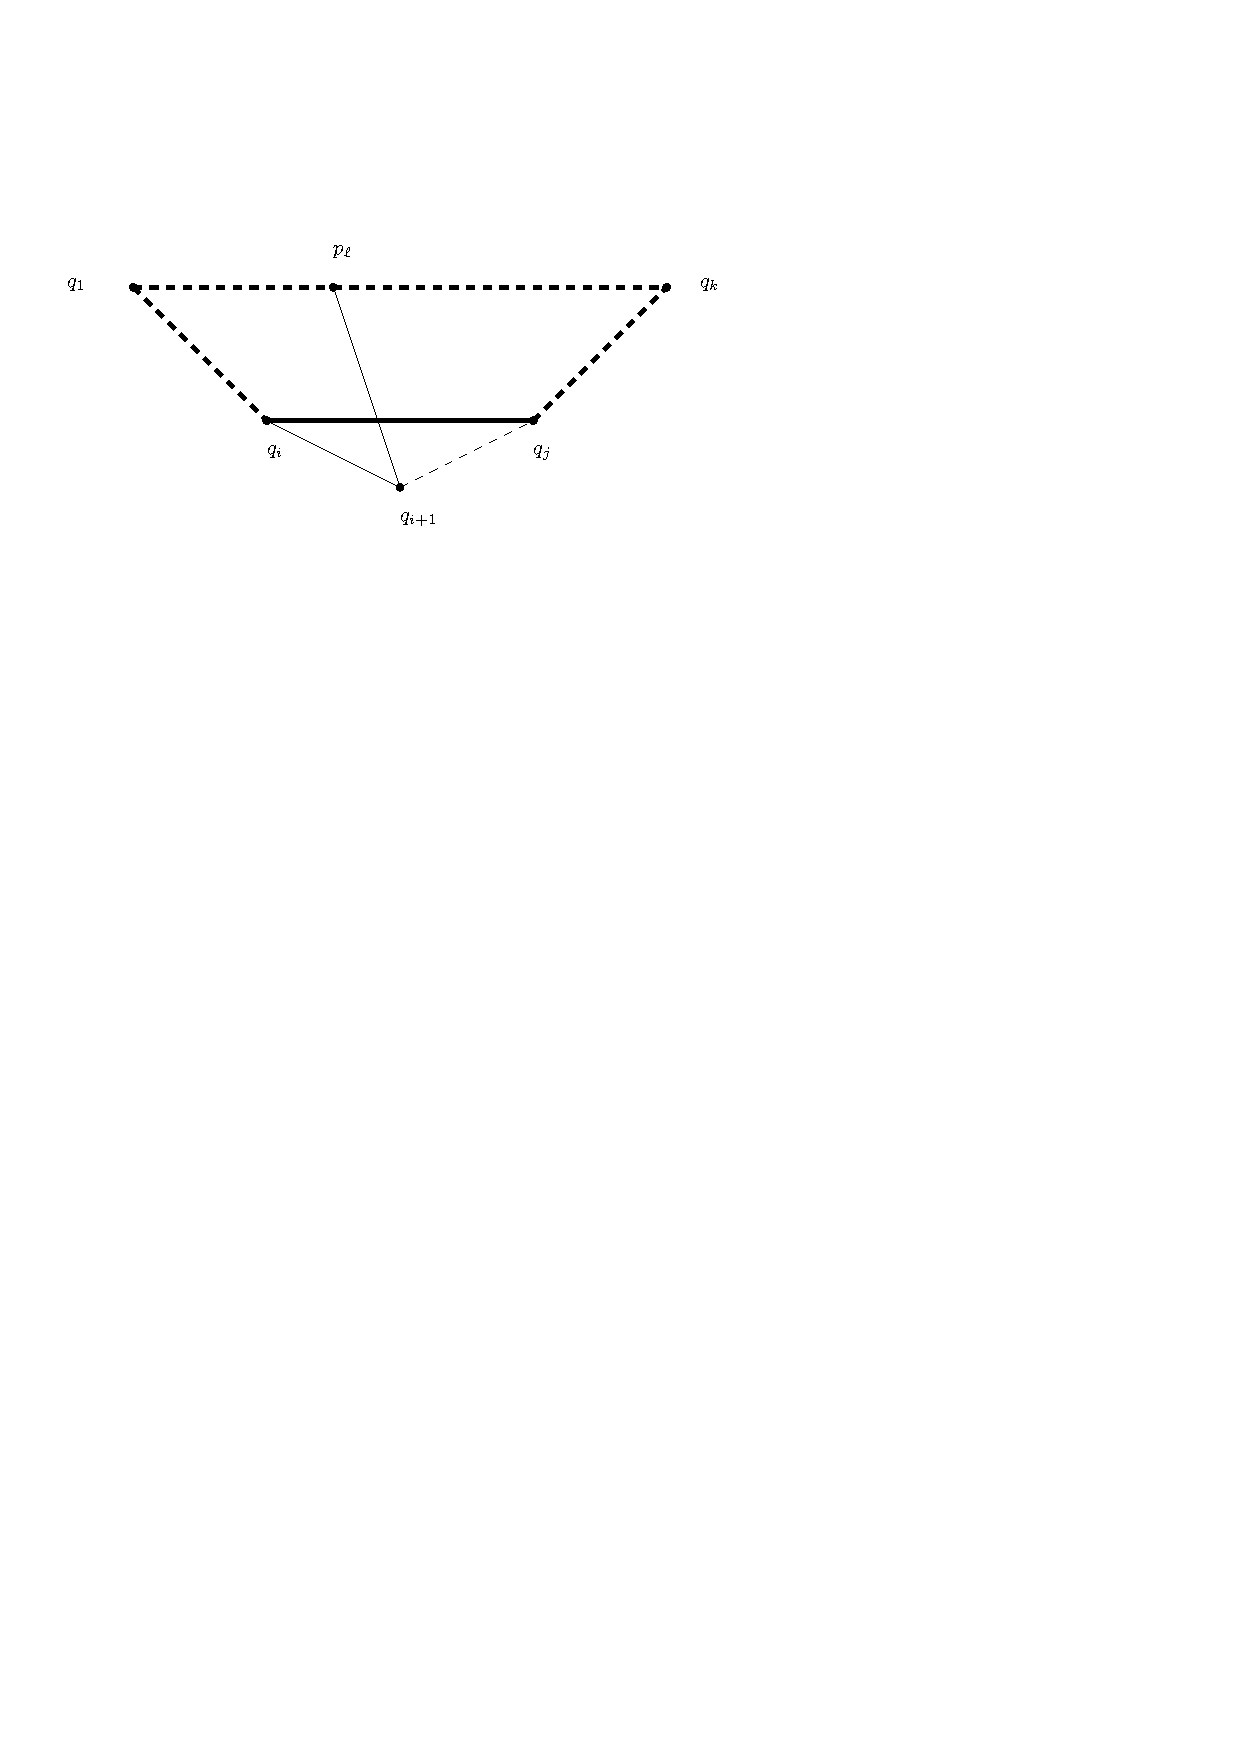
\includegraphics[scale=1]{unifiedAlgo/img/neighbourWalkChords}
      \caption{The construction in the proof of Lemma \ref{lm:uni:neighbourwalkChordFree}}
      \label{fig:uni:neihbourwalkChordFree}
    \end{figure}
  \end{proof}

  \fxnote{Alternate proof based on   ($\W$ being oriented from $\pW$ to $\pE$), since if it would lie on the left of $\W$ the vertices $w_{i+1},\ldots, w_{j-1}$ would not have been chosen in the construction of the prefence.}
